% autore: Matilde Padovano

Potremmo pensare che per risolvere il problema sia sufficiente costruire un array, per cui ogni elemento  di indice $x$ contiene il numero di volte che una pagina compare con il numero $x$ e restituire l'elemento il cui valore è $1$. Questa soluzione può risolvere i primi subtask, ma nel ultimo il numero delle pagine può arrivare fino a $1000000000$, è quindi impossibile risolvere il problema con questa soluzione per via la troppa memoria usata.\itemize
Per risolvere anche l'ultimo subtask, dobbiamo controllare direttamente dall'array $P$ quale elemento compare una sola volta.  Per farlo è necessario ordinare $P$.  A questo punto è sufficiente controllare per ogni coppia, spostandoci di 2 posizioni ogni volta, se gli elementi sono uguali. Se non lo sono vuol dire che il primo elemeto della coppia compare solo una volta. Possiamo quindi restituire quest ultimo.\itemize\newline
Esempio:\newline
$P$: 5 6 5 7 9 6 8 9 7\itemize\newline
$P$ dopo averlo ordinato:  5 5 6 6 7 7 8 9 9\itemize \newline
coppie da contollare:  5-5;6-6;7-7;8-9; 8 è diverso da 9, quindi è il numero spaiato \itemize

\colorbox{white}{\makebox[.99\textwidth][l]{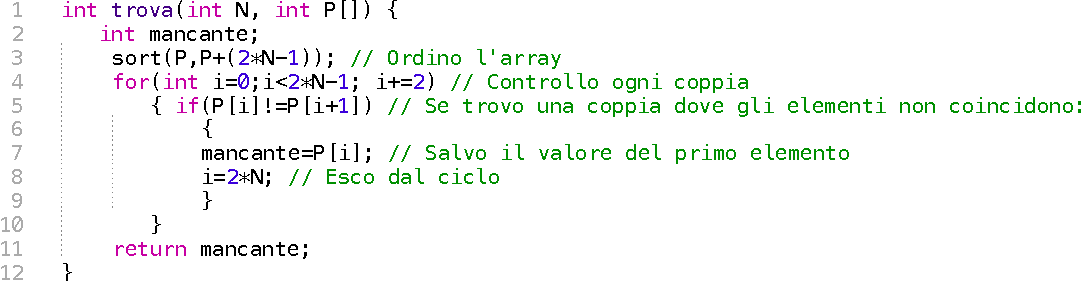
\includegraphics[scale=.8]{duplicato.pdf}}} 